% fig5.tex — Program embedding landscape (Observation 4)
% Generated from fig5.html via Puppeteer → fig5.pdf

\begin{figure*}[t]
\centering
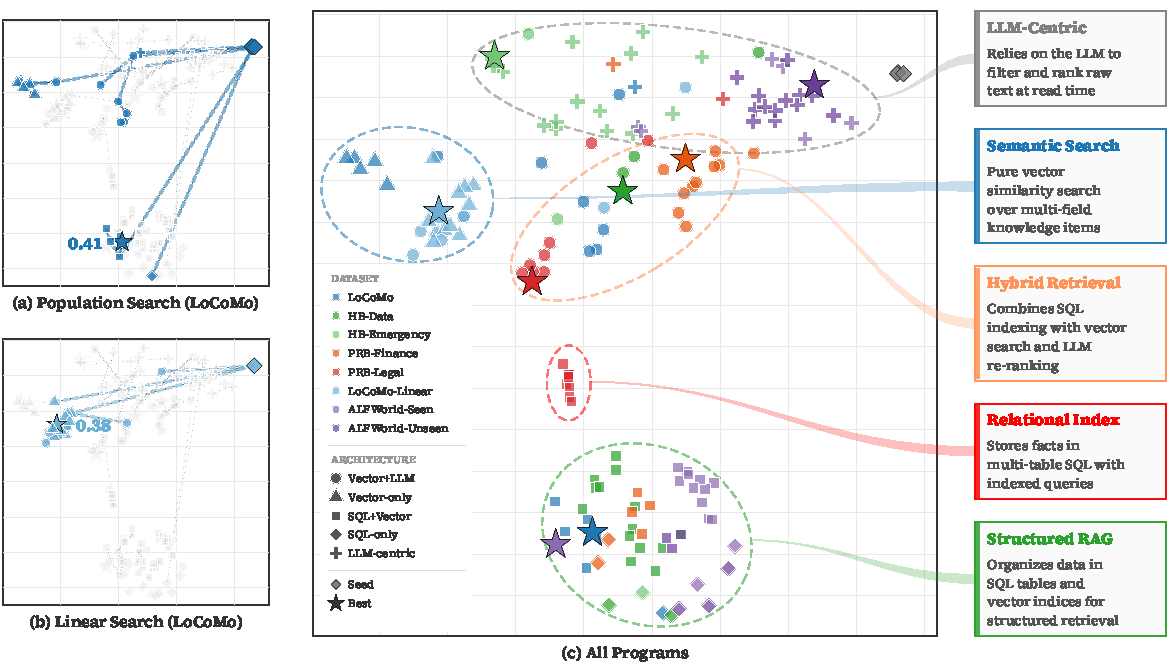
\includegraphics[width=\textwidth]{figures/landscape/fig5.pdf}
\caption{%
  \textbf{Program embedding landscape.}
  Each evolved program is embedded with a code embedding model and projected to 2D via t-SNE~\citep{vandermaaten2008tsne}.
  \textbf{(a,\,b)}~Population-based search (\sysname{}) and linear search, with colored edges tracing parent-child lineage.
  \textbf{(c)}~All programs from the evaluated configurations and the LoCoMo linear-search ablation, colored by configuration.
  Marker shapes denote the storage architecture discovered by evolution: circles for vector\,+\,LLM, triangles for vector-only, squares for SQL\,+\,vector, rotated squares for SQL-only, and crosses for LLM-centric designs; diamonds mark seed programs and stars mark the best program for each configuration.
}
\label{fig:landscape}
\end{figure*}
